\subsection{Use Case}
\begin{figure}[H]
\label{fig:uc2}
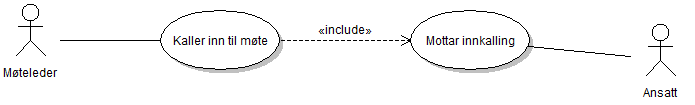
\includegraphics[width=400px]{ucs2.png}
\caption{Use Case-diagram for scenario 2}
\end{figure}

\subsection{Tekstlig Use Case}
\begin{table}[H]
\centering
\label{tab:tuc2}
\begin{tabular}{| l | L{4in} |}
\hline
Use Case & Scenario 2 \\
\hline
Aktør & Møteleder og inviterte ansatte \\
\hline
Trigger & Møteleder inviterer ansatte til et møte \\
\hline
Pre-betingelser & Møteleder har laget møtet \\
\hline
Post-betingelser & Ansatte er invitert til møtet, og mottar melding om dette når de logger seg på systemet. \\
\hline
Normal hendelsesflyt & 
\begin{minipage}{4in}
\vskip 4pt
\begin{itemize}
\item Møteleder opprettet møtet
\item Møteleder inviterer ansatte til møtet
\item Melding blir sendt til de inviterte, som de mottar neste gang de logger seg på
\end{itemize}
\vskip 4pt
\end{minipage}
 \\
\hline
Variasjoner & \\
\hline
Relatert informasjon & De inviterte medlemmene ser meldingen neste gang de logger seg på systemet. \\
\hline
\end{tabular}
\caption{Tekslig Use Case-diagrame}
\end{table}

\subsection{Sekvensdiagram}
\begin{figure}[H]
\label{fig:sek2}
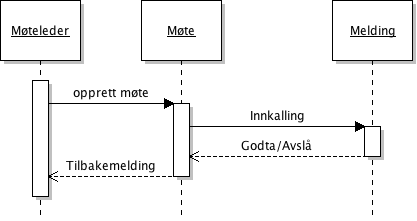
\includegraphics[width=400px]{sekvens2.png}
\caption{Use Case-diagram for scenario 2}
\end{figure}